\section{Modellierung der Daten}
\subsection{Darstellung der Klassen}
In diesem Kapitel geht es um die objektorientierte Analyse der in dem letzten Kapitel spezifizierten Anforderungen. Ziel ist es mithilfe eines Klassendiagramms die Daten des Systems visuell darzustellen und die Beziehungen der Klassen untereinander zu modellieren. Diese Klassendiagramme sollen einen tatsächlichen Aufbau des Systems darstellen, der einem späteren, nicht im Rahmen dieser Arbeit angefertigten, Entwurf und Implementierung als Vorlage dienen soll, um die tatsächlichen Klassen aufzubauen. Da dieses Klassendiagramm bereits in der Konzeptionsphase des Systems aufgebaut wird, haben diese Modellierungen keinen Anspruch auf Richtigkeit, da aus technischen oder organisatorischen Gründen zu einem späteren Zeitpunkt noch Änderungen erfolgen können. Diese Änderungen können zum Beispiel aufgrund von technischen Restriktionen der Entwicklungsumgebung oder aufgrund von Wünschen des Auftraggebers auftreten.
\\Um die Übersichtlichkeit zu bewahren wird als Erstes ein Übersichtsklassendiagramm gezeigt, dass die Klassen nur bei ihrem Namen nennt und die Beziehung zwischen den Klassen darstellt. Zuerst erfolgt die Beschreibung der Klassen und den herrschenden Assoziationen, Aggregationen, Kompositionen und Generalisierungen. Im Anschluss erfolgt die vollständige Darstellung der Klassen in einem erweiterten Klassendiagramm, in dem zusätzlich die Operationen und Attribute dargestellt sind. Danach werden die Attribute und Operationen exemplarisch anhand von drei ausgewählten Klassen spezifiziert. Zum Ende dieses Kapitels erfolgt die Zusammenfassung der Klassen zu Paketen in einem Paketdiagramm.    

\newpage
\subsection{Übersichtsklassendiagramm}
\begin{figure}[h!]
    \centering
    \includegraphics[scale=0.6]{./Bilder/Übersichtsklassendiagramm.png}
    \caption[Übersichtsklassendiagramm]{Übersichtsklassendiagramm}
    \label{fig:Übersichtsklassendiagramm}
\end{figure}
\emph{Zur verbesserten Anschauung ist das Diagramm ebenfalls im Verzeichnis ./Bilder/Übersichtsklassendiagramm.png dieser Arbeit abgelegt.}

\newpage
\subsection{Klassen und Beziehungen}
\subsubsection{Beschreibung der Klassen}
In den nachfolgenden Tabellen werden zuerst die ermittelten Klassen beschrieben, danach die Beziehungen mit Assoziationen und die Beziehungen mit Generalisierungen.

\begin{xltabular}{\textwidth}{|p{0.3\textwidth}|p{0.642\textwidth}|}
    \hline
    \textbf{Klasse} & \textbf{Beschreibung} \\\hline\hline
    Benutzer & Eine natürliche Person, die ein Benutzerkonto im System hat.\\\hline
    Administrator & Eine natürliche Person, die für die Verwaltung des Systems zuständig ist. \\\hline
    Projektleiter & Eine natürliche Person, die ein S/4HANA-Transformationsprojekt leitet. \\\hline
    Teilprojektleiter & Eine natürliche Person, die ein Teilprojekt in einem S/4HANA-Transformationsprojekt leitet. \\\hline
    Projektmitarbeiter & Eine natürliche Person, die Mitarbeiter in einem S/4HANA-Transformationsprojekt ist. \\\hline
    Kunde &  Eine natürliche Person, die Kunde eines S/4HANA-Transformationsprojekt ist.\\\hline
    Projekt & Eine Einheit, die ein S/4HANA-Transformationsprojekt abbildet. \\\hline
    Teilprojekt & Eine Einheit, die ein Teilprojekt in einem S/4HANA-Transformationsprojekt abbildet. \\\hline
    Projektphase & Ein Zeitraum in einem S/4HANA-Transformationsprojekt\\\hline
    Kriterium & Eine Eigenschaft einer Projektphase, die während der S/4HANA-Transformation erfüllt wird. \\\hline
    BoolschesKriterium & Ein Kriterium, das einen Ja- oder Nein-Wert speichert.\\\hline
    Textkriterium & Ein Kriterium, das eine Zeichenkette speichert.\\\hline
    Zahlenkriterium & Ein Kriterium, das eine Ganzzahl oder Gleitkommazahl speichert. \\\hline
    Prozess &  Ein in SAP abgebildete Folge von Aktivitäten.\\\hline
    Subprozess &  Ein in sich geschlossener Abschnitt eines Prozess.\\\hline
    Prozessschritt & Eine Aktivität eines Prozess.\\\hline
\end{xltabular}
\captionof{table}[Klassenbeschreibungen]{Beschreibung der ermittelten Klassen}

\subsubsection{Beschreibung der Assoziationen}
Assoziationen sind Beziehungen, die zwischen Klassen bestehen und können unterschiedlicher Natur sein. Assoziationen sind bidirektional und funktionieren deswegen in beide Richtungen.\\
\begin{xltabular}{\textwidth}{|p{0.3\textwidth}|p{0.145\textwidth}|p{0.145\textwidth}|p{0.3\textwidth}|}
    \hline
    \multicolumn{4}{|c|}{\textbf{Klassen mit Assoziationen}}\\\hline\hline
    %%%%%%
    Administrator & 1 & 0..* & Projekt\\\hline
    \multicolumn{4}{|p{0.942\textwidth}|}{Ein Administrator kann kein, oder mehrere Projekte im System erstellen, aber ein Projekt kann nur von genau einem Administrator erstellt werden.}\\\hline\hline
    %%%%%%
    %%%%%%
    Benutzer & 1..* & 0..* & Projekt\\\hline
    \multicolumn{4}{|p{0.942\textwidth}|}{Ein Benutzer kann kein, oder mehreren Projekten im System zugeordnet sein und ein Projekt kann keinem, oder mehreren Benutzern zugeordnet werden.}\\\hline\hline
    %%%%%%
    %%%%%%
    Administrator & 1..* & 0..* & Benutzer\\\hline
    \multicolumn{4}{|p{0.942\textwidth}|}{Ein Administrator kann ein, keinen, oder mehrere Benutzer verwalten und ein Benutzer kann von einem, oder mehreren Administratoren verwaltet werden.}\\\hline\hline
    %%%%%%
    Projektleiter & 1..* & 1 & Projektphase\\\hline
    \multicolumn{4}{|p{0.942\textwidth}|}{Ein Projektleiter kann eine, oder mehrere Projektphasen erstellen, aber eine Projektphase kann nur durch genau einen Projektleiter erstellt werden.}\\\hline\hline
    %%%%%%
    %%%%%%
    Teilprojektleiter & 1 & 0..* & Kriterium\\\hline
    \multicolumn{4}{|p{0.942\textwidth}|}{Ein Teilprojektleiter kann kein, oder beliebig viele Kriterien erstellen, ein Kriterium wird jedoch nur durch eine Teilprojektleiter erstellt.}\\\hline\hline
    %%%%%%
    Projektleiter & 1..* & 0..* & Projekt\\\hline
    \multicolumn{4}{|p{0.942\textwidth}|}{Ein Projektleiter verwaltet kein, oder mehrere Projekte und ein Projekt wird durch mindestens einen Projektleiter verwaltet}\\\hline\hline
    %%%%%%
    Teilprojektleiter & 1..* & 0..* & Teilprojekt\\\hline
    \multicolumn{4}{|p{0.942\textwidth}|}{Ein Teilprojektleiter verwaltet kein, oder mehrere Teilprojekte und ein Teilprojekt wird durch mindestens einen Projektleiter verwaltet}\\\hline\hline
    %%%%%%
    Projektmitarbeiter & 1 & 0..* & Kriterium\\\hline
    \multicolumn{4}{|p{0.942\textwidth}|}{Ein Projektmitarbeiter kann kein, oder beliebig viele Kriterien erstellen, ein Kriterium wird jedoch nur durch einen Projektmitarbeiter erstellt.}\\\hline\hline
    Prozessschritt & 0..* & 0..* & Kriterium\\\hline
    \multicolumn{4}{|p{0.942\textwidth}|}{Ein Prozessschritt prägt kein, oder beliebig viele Kriterien aus und ein Kriterium wird durch kein, oder beliebig vielen Prozessschritten ausgeprägt.}\\\hline\hline
    Kunde & 0..* & 0..1 & Projekt\\\hline
    \multicolumn{4}{|p{0.942\textwidth}|}{Ein Kunde betrachtet keins, oder ein Projekt und ein Projekt wird von keinem, oder mehreren Kunden betrachtet.}\\\hline\hline
    Subprozess & 0..1 & 1..* & Prozessschritt\\\hline
    \multicolumn{4}{|p{0.942\textwidth}|}{Ein Subprozess beinhaltet einen, oder mehrere Prozessschritte und ein Prozessschritt kann zu keinem, oder einem Prozessschritt gehören, da Subprozesse nur optional sind.}\\\hline
    
\end{xltabular}
\captionof{table}[Klassen mit Assoziationen]{Beschreibung der ermittelten Klassen mit Assoziationen}

\newpage
\subsubsection{Beschreibung der Aggregationen}
Aggregationen sind eine besondere Form von Assoziationen, bei denen Objekte einer Klasse einen Teil von einer anderen Klasse darstellen. Dadurch ist es möglich beispielsweise Besitz darzustellen.\\

\begin{xltabular}{\textwidth}{|p{0.3\textwidth}|p{0.145\textwidth}|p{0.145\textwidth}|p{0.3\textwidth}|}
    \hline
    \multicolumn{4}{|c|}{\textbf{Klassen mit Aggregationen}}\\\hline\hline
    Teilprojekt & 1..* & 0..* & Prozess\\\hline
    \multicolumn{4}{|p{0.942\textwidth}|}{Ein Teilprojekt beinhaltet keinen oder mehrere Prozesse, ein Prozess gehört aber immer zu einem oder mehreren Teilprojekten. Ein Teilprojekt ohne Prozesse kann existieren, ein Prozess ohne nicht mindestens ein Teilprojekt jedoch nicht.}\\\hline\hline
    Teilprojekt & 1 & 0..1 & Projektmitarbeiter\\\hline
    \multicolumn{4}{|p{0.942\textwidth}|}{Ein Teilprojekt hat keinen oder mehrere zugeordnete Projektmitarbeiter und ein Projektmitarbeiter ist immer einem Teilprojekt zugeordnet. Ein Teilprojekt ohne Projektmitarbeiter kann existieren, ein Projektmitarbeiter ohne Teilprojekt jedoch nicht.}\\\hline\hline
    Prozess & 1 & 0..* & Subprozess\\\hline
    \multicolumn{4}{|p{0.942\textwidth}|}{Ein Prozess kann keine oder mehrere Subprozesse beinhalten, ein Subprozess gehört immer zu genau einem Prozess. Ein Prozess ohne Subprozesse kann existieren, ein Subprozess ohne Prozess jedoch nicht.}\\\hline
\end{xltabular}
\captionof{table}[Klassen mit Aggregation]{Beschreibung der ermittelten Klassen mit Aggregationen}
\newpage
\subsubsection{Beschreibung der Kompositionen}
Kompositionen sind eine besondere Form von Aggregation, bei denen die Objekte der einen Klasse nicht ohne die Objekte der anderen Klasse existieren können.\\

\begin{xltabular}{\textwidth}{|p{0.3\textwidth}|p{0.145\textwidth}|p{0.145\textwidth}|p{0.3\textwidth}|}
    \hline
    \multicolumn{4}{|c|}{\textbf{Klassen mit Kompositionen}}\\\hline\hline
    Projekt & 1 & 1..5 & Projektphase\\\hline
    \multicolumn{4}{|p{0.942\textwidth}|}{Ein Projekt kann eine, oder bis zu fünf Projektphasen beinhalten und eine Projektphase gehört immer zu genau einem Projekt. Ein Projekt ohne Projektphasen kann nicht existieren, eine Projektphase ohne Projekt ebenfalls nicht.}\\\hline\hline
    %%%%%%
    Projekt & 1 & 1..* & Teilprojekt\\\hline
    \multicolumn{4}{|p{0.942\textwidth}|}{Ein Projekt kann ein, oder mehrere Teilprojekte beinhalten und ein Teilprojekt gehört zu genau einem Projekt. Ein Projekt ohne Teilprojekte kann nicht existieren, ein Teilprojekt ohne Projekt ebenfalls nicht.}\\\hline\hline
    %%%%%%
    Projektphase & 1 & 1..* & Kriterium\\\hline
    \multicolumn{4}{|p{0.942\textwidth}|}{Eine Projektphase hat ein, oder mehrere Kriterien und ein Kriterium gehört zu genau einer Projektphase. Eine Projektphase ohne Kriterien kann nicht existieren, ein Kriterium ohne Projektphase ebenfalls nicht.}\\\hline\hline
    %%%%%%
    Prozess & 1 & 1..* & Prozessschritt\\\hline
    \multicolumn{4}{|p{0.942\textwidth}|}{Ein Prozess hat ein, oder mehrere Prozessschritte und ein Prozessschritt gehört immer zu genau einem Prozess. Ein Prozess ohne Prozessschritte kann nicht existieren, ein Prozessschritt ohne Prozess ebenfalls nicht.}\\\hline
    %%%%%%
\end{xltabular}
\captionof{table}[Klassen mit Kompositionen]{Beschreibung der ermittelten Klassen mit Kompositionen}
\newpage
\subsubsection{Beschreibung der Generalisierungen}
Generalisierungen sind Vererbungsbeziehungen, bei denen es eine Basisklasse gibt, die ihre Kriterien an eine oder mehrere spezialisierte, bzw. abgeleitete Klassen vererbt.\\

\begin{xltabular}{\textwidth}{|p{0.472\textwidth}|p{0.472\textwidth}|}
    \hline
    \multicolumn{2}{|c|}{\textbf{Klassen mit Generalisierungen}}\\\hline\hline
    BoolschesKriterium, Textkriterium, Zahlenkriterium & Kriterium \\\hline
    \multicolumn{2}{|p{0.944\textwidth}|}{Die Klasse Kriterium ist abstrakt und vererbt ihre Eigenschaften an die abgeleiteten Klassen BoolschesKriterium, Textkriterium und Zahlenkriterium.}\\\hline\hline
    Administrator, Projektleiter, Teilprojektleiter, Projektmitarbeiter, Kunde & Benutzer \\\hline
    \multicolumn{2}{|p{0.944\textwidth}|}{Die Klasse Benutzer ist abstrakt und vererbt ihre Eigenschaften an die abgeleiteten Klassen Administrator, Projektleiter, Teilprojektleiter, Projektmitarbeiter und Kunde.}\\\hline
\end{xltabular}
\captionof{table}[Klassen mit Generalisierungen]{Beschreibung der ermittelten Klassen mit Generalisierungen}
\newpage
\subsection{Erweitertes Klassendiagramm}
\begin{figure}[h!]
    \centering
    \includegraphics[scale=0.45]{./Bilder/GroßesKlassendiagramm.png}
    \caption[Erweitertes Klassendiagramm]{Erweitertes Klassendiagramm}
    \label{fig:Klassendiagramm}
\end{figure}
\emph{Zur verbesserten Anschauung ist das Diagramm ebenfalls im Verzeichnis ./Bilder/Klassendiagramm.png dieser Arbeit abgelegt.}
\newpage
\subsection{Detaillierte Spezifikationen der Klassen}
Nachfolgend werden zur Begründung des Vorgehens im erweiterten Klassendiagramm, exemplarisch die Attribute, Operationen und strukturierten Datentypen der Klassen Benutzer, Projekt und Prozessschritt genauer spezifiziert. Dazu werden die Attribute der Klassen und die Attribute der strukturierten Datentypen anhand der Kriterien \glqq{}Datentyp\grqq{}, \glqq{}Anfangswert\grqq{}, \glqq{}Erforderlichkeit\grqq{}, \glqq{}Schlüssel\grqq{}, \glqq{}Änderbarkeit\grqq{}, \glqq{}Einheit\grqq{}, und \glqq{}Beschreibung\grqq{} beschrieben und aufgeschlüsselt, sowie die Operationen anhand der Eigenschaften \glqq{}Typ\grqq{}, \glqq{}Parameter\grqq{}, \glqq{}Ergebnis\grqq{} und \glqq{}Wirkung\grqq{}. 

\subsubsection{Spezifikationen der Klasse Benutzer}
\begin{xltabular}{\textwidth}{|p{0.155\textwidth}||P{0.1\textwidth}|P{0.11\textwidth}|P{0.1\textwidth}|P{0.12\textwidth}|P{0.11\textwidth}|P{0.105\textwidth}|}
    \hline
    \multicolumn{7}{|c|}{\textbf{Attribute der Klasse Benutzer}}\\\hline
    Attribut & user & passwort & vorname & nachname & abteilung & userID\\\hline\hline
    Datentyp & String & String & String & String & String & String\\\hline
    Anfangswert & - & - & - & - & - & USR0001\\\hline
    Erforderlich & ja & ja & nein & nein & nein & ja \\\hline
    Schlüssel & ja & nein & nein & nein & nein & ja\\\hline
    Änderbarkeit & ja & ja & ja & ja & ja & nein \\\hline
    Einheit & - & - & - & - & - & -\\\hline
    Beschreibung & - & Nur durch Benutzer festlegbar & - & - & - & - \\\hline
\end{xltabular}
\captionof{table}[Klassenattribute Benutzer]{Attribute der Klasse Benutzer}
\newpage
\begin{xltabular}{\textwidth}{|p{0.18\textwidth}||P{0.13\textwidth}|P{0.15\textwidth}|P{0.16\textwidth}|P{0.24\textwidth}|}
    \hline
    \multicolumn{5}{|c|}{\textbf{Operationen der Klasse Benutzer}}\\\hline
    Operation & Typ & Parameter & Ergebnis & Wirkung\\\hline\hline
    gibStammdaten & Objekt-operation & userID: String & StammdatenT & User, Name, Abteilung und ID werden ausgegeben\\\hline
    gibBenutzerrolle & Objekt-operation & userID: String & String & Benutzerrolle wird ausgegeben\\\hline
    erstelleBenutzer & Klassen-operation & user: String & String & Neuer Benutzer wird erstellt, ID zurückgegeben\\\hline
    sperreBenutzer & Objekt-operation & userID: String & - & Der Zugang des Benutzers wird gesperrt\\\hline
    gibID & Objekt-operation & user: String & String & ID des Benutzers wird ausgegeben\\\hline
\end{xltabular}
\captionof{table}[Klassenoperationen Benutzer]{Operationen der Klasse Benutzer}
\vspace{5em}
\begin{xltabular}{\textwidth}{|p{0.17\textwidth}||P{0.14\textwidth}|P{0.14\textwidth}|P{0.13\textwidth}|P{0.13\textwidth}|P{0.13\textwidth}|}
    \hline
    \multicolumn{6}{|c|}{\textbf{Strukturierer Datentyp StammdatenT}}\\\hline
    Attribut & user & vorname & nachname & abteilung & userID\\\hline\hline
    Datentyp & String & String & String & String & String\\\hline
    Anfangswert & - & - & - & - & -\\\hline
    Erforderlich & ja & nein & nein & nein & ja \\\hline
    Schlüssel & ja & nein & nein & nein & ja\\\hline
    Änderbarkeit & ja & ja & ja & ja & nein \\\hline
    Einheit & - & - & - & - & -\\\hline
    Beschreibung & - &  - & - & - & - \\\hline
\end{xltabular}
\captionof{table}[Strukturierter Datentyp StammdatenT]{Strukturierter Datentyp StammdatenT}
\vspace{3em}
\subsubsection{Spezifikationen der Klasse Projekt}
\begin{xltabular}{\textwidth}{|p{0.15\textwidth}||P{0.09\textwidth}|P{0.11\textwidth}|P{0.08\textwidth}|P{0.085\textwidth}|P{0.095\textwidth}|P{0.095\textwidth}|P{0.08\textwidth}|}
    \hline
    \multicolumn{8}{|c|}{\textbf{Attribute der Klasse Projekt}}\\\hline
    Attribut & prjname & prjID & kunde & beschrb & beginn & ende & prjleit\\\hline\hline
    Datentyp & String & String & String & String & DatumT & DatumT & String \\\hline
    Anfangswert & - & PRJ0001 & - & - & 01.01.21 & 01.01.22 & - \\\hline
    Erforderlich & ja & ja & ja & nein & ja & nein & ja \\\hline
    Schlüssel & nein & ja & nein & nein & nein & nein & nein \\\hline
    Änderbarkeit & ja & nein & ja & ja & nein & ja & ja\\\hline
    Einheit & - & - & - & - & Zeit & Zeit & - \\\hline
    Beschreibung & - & - & - & Freitext & - & - & -\\\hline
\end{xltabular}
\captionof{table}[Klassenattribute Projekt]{Attribute der Klasse Projekt}
\vspace{5em}
\begin{xltabular}{\textwidth}{|p{0.22\textwidth}||P{0.13\textwidth}|P{0.15\textwidth}|P{0.16\textwidth}|P{0.22\textwidth}|}
    \hline
    \multicolumn{5}{|c|}{\textbf{Operationen der Klasse Projekt}}\\\hline
    Operation & Typ & Parameter & Ergebnis & Wirkung\\\hline\hline
    erstelleProjekt & Klassen-operation & prjname: String & String & Neues Projekt wird erstellt, ID zurückgegeben \\\hline
    gibFortschritt & Objekt-operation & prjID: String & float & Der Gesamtfortschritt in Prozent wird ausgegeben \\\hline
    gibTeilprojekte & Objekt-operation & prjID: String & String[] & Es wird ein Array mit den Teilprojekten Ausgegeben \\\hline
    ändereProjektleiter & Objekt-operation & prjID: String; prjleit: String & - & Projektleiter wird geändert \\\hline
    ändereEnde & Objekt-operation & ende: DatumT & - & Die Laufzeit wird verländert \\\hline
    gibID & Objekt-operation & prjname: String & String & ID des Projekts wird ausgegeben\\\hline
\end{xltabular}
\captionof{table}[Klassenoperationen Projekt]{Operationen der Klasse Projekt}
\vspace{3em}
\begin{xltabular}{\textwidth}{|p{0.23\textwidth}||P{0.23\textwidth}|P{0.23\textwidth}|P{0.23\textwidth}|}
    \hline
    \multicolumn{4}{|c|}{\textbf{Strukturierer Datentyp DatumT}}\\\hline
    Attribut & tag & monat & jahr\\\hline\hline
    Datentyp & int & int & int\\\hline
    Anfangswert & 1 & 1 & 2021 \\\hline
    Erforderlich & ja & ja & ja\\\hline
    Schlüssel & ja & ja & ja\\\hline
    Änderbarkeit & ja & ja & ja\\\hline
    Einheit & Tage & Monat & Jahr\\\hline
    Beschreibung & - & - & -\\\hline
\end{xltabular}
\captionof{table}[Strukturierter Datentyp DatumT]{Strukturierter Datentyp DatumT}


\subsubsection{Spezifikationen der Klasse Prozessschritt}
\begin{xltabular}{\textwidth}{|p{0.18\textwidth}||P{0.135\textwidth}|P{0.135\textwidth}|P{0.135\textwidth}|P{0.135\textwidth}|P{0.135\textwidth}|}
    \hline
    \multicolumn{6}{|c|}{\textbf{Attribute der Klasse Prozessschritt}}\\\hline
    Attribut & schrittID & name & subprozess & prozess & teilprojekt \\\hline\hline
    Datentyp & String & String & String & String & TeilprojekT \\\hline
    Anfangswert & PSR001 & - & - & - & - \\\hline
    Erforderlich & ja & ja & nein & ja & nein\\\hline
    Schlüssel & ja & nein & nein & nein & nein\\\hline
    Änderbarkeit & nein & ja & ja & ja & ja \\\hline
    Einheit & - & - & - & - & -\\\hline
    Beschreibung & - & - & - & - & -\\\hline
\end{xltabular}
\captionof{table}[Klassenattribute Prozessschritt]{Attribute der Klasse Prozessschritt}
\vspace{3em}
\begin{xltabular}{\textwidth}{|p{0.21\textwidth}||P{0.15\textwidth}|P{0.15\textwidth}|P{0.15\textwidth}|P{0.225\textwidth}|}
    \hline
    \multicolumn{5}{|c|}{\textbf{Operationen der Klasse Prozessschritt}}\\\hline
    Operation & Typ & Parameter & Ergebnis & Wirkung\\\hline\hline
    gibProzess & Objekt-operation & schrittID: String & String & ID des Prozess wird ausgegeben\\\hline
    gibSubprozess & Objekt-operation & schrittID: String & String & ID des Subprozess wird ausgegeben\\\hline
    erstelleSchritt & Klassen-operation & name: String; prozess: String & String & Neuer Schritt wird angelegt; ID wird zurückgegeben\\\hline
    gibFortschritt & Objekt-operation & schrittID: String & float & Fortschritt des Schritts wird in Prozent ausgegeben \\\hline
    gibID & Objekt-operation & name: String & String & ID des Schritts wird ausgegeben\\\hline
\end{xltabular}
\captionof{table}[Klassenoperationen Prozessschritt]{Operationen der Klasse Prozessschritt}
\vspace{3em}
\begin{xltabular}{\textwidth}{|p{0.23\textwidth}||P{0.23\textwidth}|P{0.23\textwidth}|P{0.23\textwidth}|}
    \hline
    \multicolumn{4}{|c|}{\textbf{Strukturierer Datentyp TeilprojektT}}\\\hline
    Attribut & name & teilprojektID & prjID\\\hline\hline
    Datentyp & String & String & String\\\hline
    Anfangswert & - & TPR0001 & PRJ0001 \\\hline
    Erforderlich & ja & ja & ja\\\hline
    Schlüssel & nein & ja & ja\\\hline
    Änderbarkeit & ja & ja & ja\\\hline
    Einheit & - & - & -\\\hline
    Beschreibung & - & - & -\\\hline
\end{xltabular}
\captionof{table}[Strukturierter Datentyp TeilprojektT]{Strukturierter Datentyp TeilprojekT}
\newpage
\subsection{Paketdiagramm}
Die nachfolgende Abbildung zeigt die Bündelung der ermittelten Klassen des Business Transformation Trackers zu vier Paketen in einem Paketdiagramm.\\
\begin{figure}[h!]
    \centering
    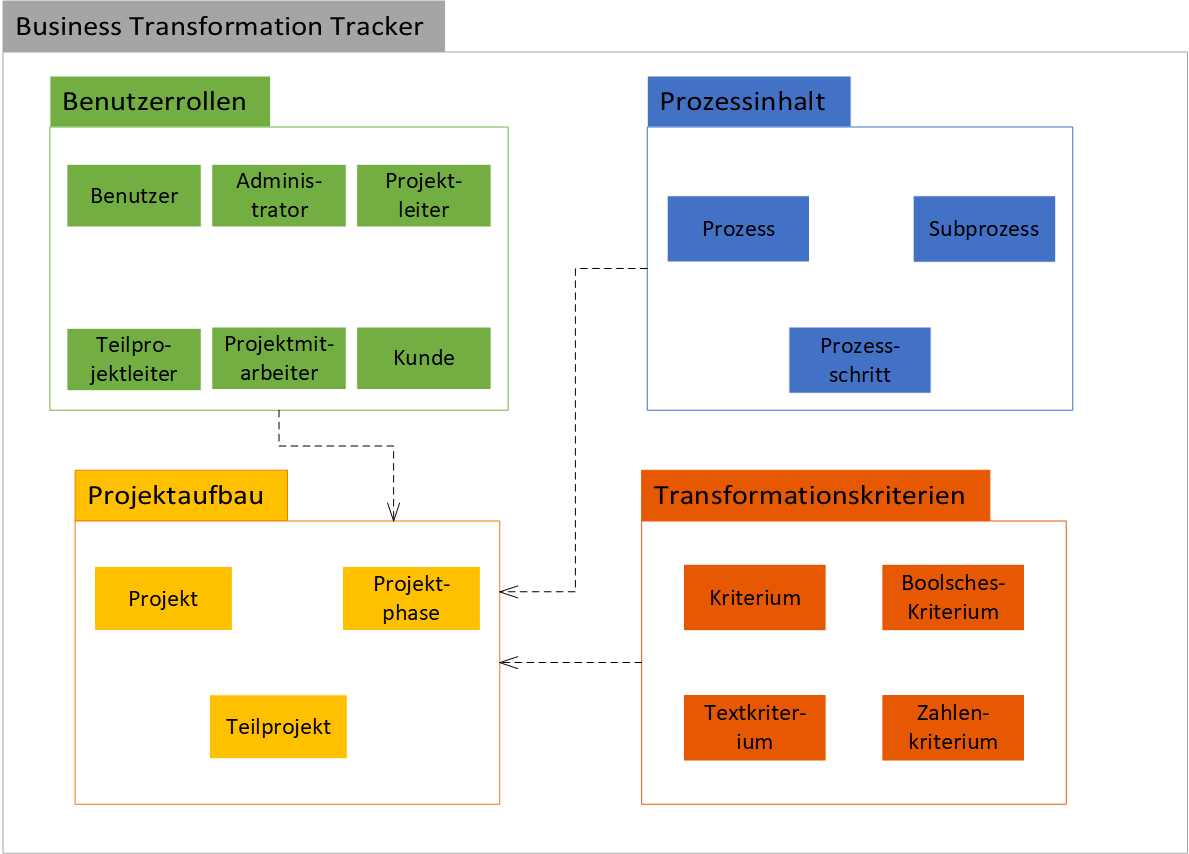
\includegraphics[scale=0.8]{./Bilder/Paketdiagramm.png}
    \caption[Paketdiagramm]{Paketdiagramm}
    \label{fig:Paketdiagramm}
\end{figure}
\\Die ermittelten Pakete sind \glqq{}Benutzerrollen\grqq{}, \glqq{}Projektaufbau\grqq{}, \glqq{}Prozessinhalt\grqq{} und \glqq{}Transformationskriterien\grqq{}. 
\vspace{1em}
\\Das Paket \underline{Benutzerrollen} enthält die Klassen \emph{Benuter, Administrator, Projektleiter, Teilprojektleiter, Projektmitarbeiter und Kunde}. Diese Klassen werden für den Aufbau der Berechtigungen und der Rollen benötigt werden. 
\vspace{1em}
\\In dem Paket \underline{Projektaufbau} befinden sich die Klassen \emph{Projekt, Projektphase und Teilprojekt}, die im System für den Aufbau des Projektes zuständig sind. 
\vspace{1em}
\\In dem Paket \underline{Prozessinhalt} befinden sich die Klassen \emph{Prozess, Subprozess und Prozessschritt}, die in der direkten Interaktion mit dem Anwender stehen. Mit ihnen werden die Geschäftsprozesse im System erfasst, indem diese nach Prozess, Subprozess und Prozessschritt aufgespalten werden. 
\vspace{1em}
\\Das Paket \underline{Transformationskriterien} enthält die Klassen \emph{Kriterium, BoolschesKriterium, Textkriterium und Zahlenkriterium}, die für die Ausprägung der Fortschrittserfassung der Geschäfts-prozesse benötigt werden.
\vspace{1em}
\\Es bestehen Abhängigkeiten zwischen den Paketen \underline{Projektaufbau} und \underline{Prozessinhalt}; \underline{Prozessinhalt} und \underline{Transformationskriterien}; \underline{Benutzerrollen} und \underline{Projektaufbau} sowie zwischen \underline{Projektaufbau} und \underline{Transformationskriterien}. In allen Fällen ist das Paket \underline{Projektaufbau} das unabhängigste, da eine Änderung hier sich mit großer Wahrscheinlichkeit auch auf die anderen Pakete auswirkt, jedoch nicht umgekehrt.
\vspace{1em}
\\\emph{Zur verbesserten Anschauung ist das Diagramm ebenfalls im Verzeichnis ./Bilder/Paketdiagramm.png dieser Arbeit abgelegt.}
